\documentclass[./main.tex]{subfiles}

\begin{document}
\section{Preprocessamento ed analisi esplorativa}
Ciascun segnale è stato suddiviso in intervalli di ampiezza \SI{1.5}{s}, che sono stati utilizzati come unità statistiche. Dal momento che ciascuna unità è una serie storica, si è scelto di riassumerla con le seguenti variabili:
\begin{table}[H]
	\centering
	\begin{tabular}{ll}
		\texttt{minA}& minimo dell'accelerazione\\
		\texttt{medA}& mediana dell'accelerazione\\
		\texttt{varA}& varianza dell'accelerazione\\
		\texttt{maxA}& massimo dell'accelerazione\\
		\texttt{meanA}& media dell'accelerazione\\
		\texttt{MVDeriv}& media del valore assoluto della derivata seconda.
	\end{tabular}
\end{table}
Siccome i segnali di {\em shake} sono ad alta frequenza, si è scelto di utilizzare la variabile \texttt{MVDeriv} per discriminare le alte frequenze dalle basse frequenze. Infatti, \texttt{MVDeriv} assume valori grandi quando la curvatura della funzione è mediamente elevata nell'intervallo, cioé quando la frequenza è alta. L'operazione di derivazione nel punto $t$ è approssimata con\cite{NumpyGradientNumPy}
\[
\dot{a}_t = \dfrac{a_{t + 1} - a_{t - 1}}{2}\,.
\]
I dati sono stati suddivisi in insieme di stima (70\%), di convalida (15\%) e di test (15\%). Le previsioni riportate nelle conclusioni sono relative all'insieme di test, su cui è stato applicato il modello migliore valutato in termini di accuratezza sull\rq{}insieme di convalida.
In appendice sono riportate le distribuzioni marginali delle variabili riassuntive per ciascuna classe.\\

Per valutare graficamente la separabilità delle classi, l'informazione migliore è data dal t-SNE sui dati sbiancati (Figura~\ref{fig:tsne}). Le componenti principali e le componenti indipendenti, invece, non riescono a separare le classi in modo soddisfacente (Appendice A).
\begin{figure}[H]
	\centering
	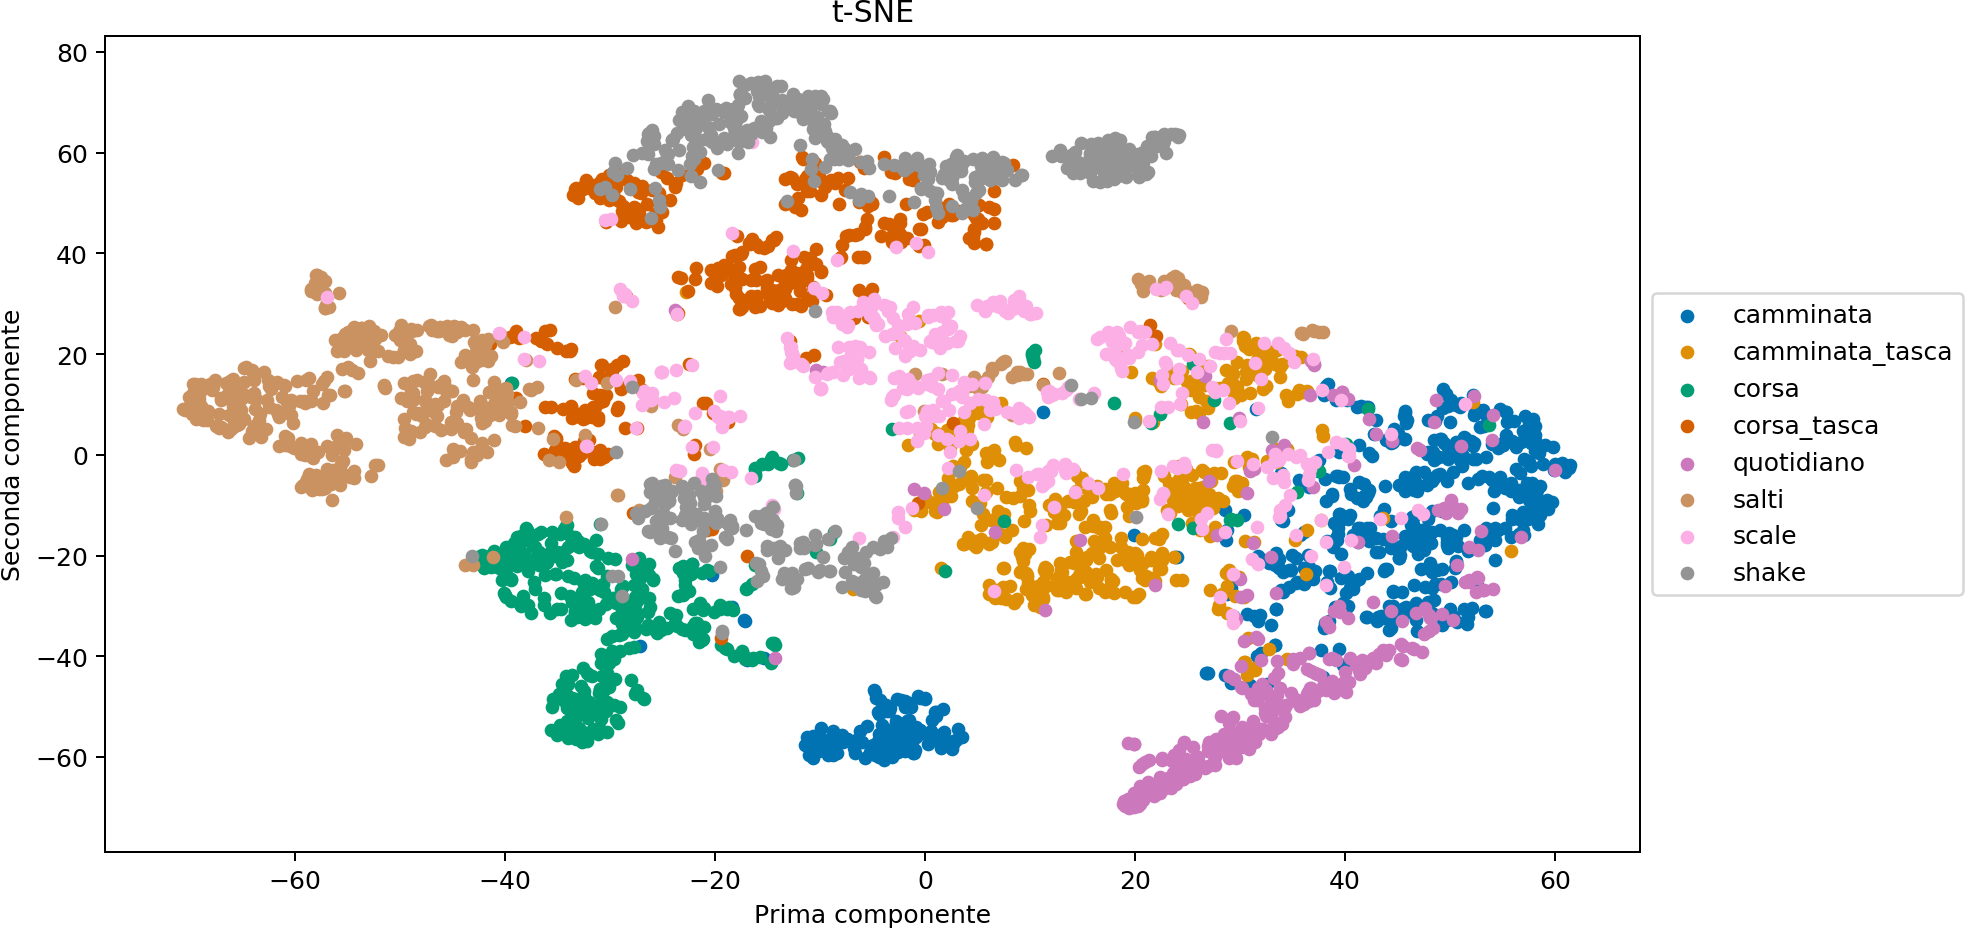
\includegraphics[width=.8\textwidth]{../../figure/t-SNE.png}
	\caption{{ t-SNE per i dati sbiancati}}
	\label{fig:tsne}
\end{figure}
\end{document}